% ════════════════════════════════════════════════════════════════
\section{Wykład 11}
\subsection{Algorytm Approx Vertex Cover (cd.)}
% ════════════════════════════════════════════════════════════════

\paragraph{Złożoność czasowa algorytmu AVC}
$n = |V(G)|$, $m = |E(G)|$.
\begin{itemize}[nosep]
	\item linia 1: $\BO(1)$
	\item linia 2: $\BO(m)$
	\item pętlę z linii 3--6 można zaimplementować, żeby działała w czasie $\BO(m)$
	\item linia 7: $\BO(1)$
\end{itemize}
Złożoność czasowa AVC wynosi $\BO(m)$.

\begin{theorem}
	AVC jest algorytmem $2$-aproksymacyjnym.
\end{theorem}
\begin{proof}
	Niech $G$ -- graf wejściowy.\\
	$c^*(G)$ -- najmniejsza liczba wierzchołków w pokryciu wierzchołkowym $G$.\\
	$c(G)$ -- liczba wierzchołków w pokryciu wierzchołkowym znalezionym przez AVC.
	
	Niech $B$ będzie zbiorem krawędzi wybranych przez AVC w linii 4.\\
	$B$ jest skojarzeniem (czyli zbiorem parami rozłącznych krawędzi), bo po wybraniu krawędzi $uv$ algorytm usuwa z $F$ wszystkie krawędzie incydentne z $u$ lub $v$.\\
	Żeby pokryć krawędzie z $B$ potrzeba co najmniej $|B|$ wierzchołków. Stąd $c^*(G) \geq |B|$.\\
	$c(G) = 2|B|$, bo algorytm dodaje do $C$ oba końce każdej krawędzi z $B$.
	\begin{flalign*}
		c(G) = 2|B| \leq 2 \cdot c^*(G) \implies \frac{c(G)}{c^*(G)} \leq 2 && &&
	\end{flalign*}
\end{proof}

Pokażemy, że ograniczenie $2$ jest osiągane. Rozważmy graf złożony z $m$ rozłącznych krawędzi:
\begin{figure}[H]
	\centering
	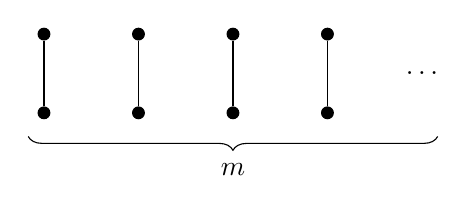
\begin{tikzpicture}[every node/.style={circle, draw, fill=black, inner sep=1.5pt}]
		\foreach \x in {0,1,2,3} {
			\node (a\x) at (\x*1.2, 1) {};
			\node (b\x) at (\x*1.2, 0) {};
			\draw (a\x) -- (b\x);
		}
		\node[draw=none, fill=none] at (4.8, 0.5) {$\ldots$};
		\draw [decorate, decoration={brace, amplitude=5pt, mirror}] (-0.2, -0.3) -- (5.0, -0.3) node[midway, draw=none, fill=none, below=5pt] {$m$};
	\end{tikzpicture}
\end{figure}
AVC zwraca pokrycie złożone z $2m$ wierzchołków, natomiast optymalne pokrycie ma rozmiar $m$ (po jednym końcu z każdej krawędzi). Stąd $\frac{c(G)}{c^*(G)} = 2$.

% ════════════════════════════════════════════════════════════════
\subsection{Problem pokrycia zbioru}
% ════════════════════════════════════════════════════════════════

\begin{definition}
	Niech $X$ -- zbiór skończony, $|X| = n$, $\mathcal{F} \subseteq 2^X$ -- rodzina podzbiorów zbioru $X$ taka, że $\bigcup_{S \in \mathcal{F}} S = X$ (każdy element $X$ należy do co najmniej jednego zbioru z $\mathcal{F}$).
	
	Rodzina $\mathcal{A} \subseteq \mathcal{F}$ jest \underline{pokryciem} zbioru $X$, jeśli $\bigcup_{S \in \mathcal{A}} S = X$.
\end{definition}

\paragraph{Przykład}
\begin{figure}[H]
	\centering
	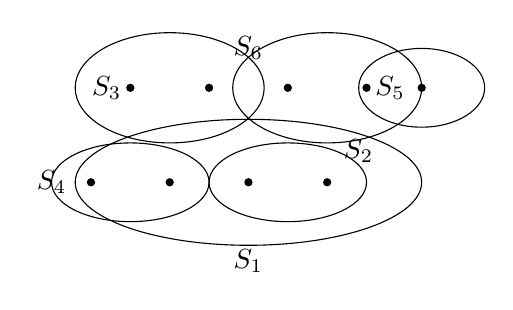
\begin{tikzpicture}
		\draw (0, 0) ellipse (2.2 and 0.8);
		\draw (-1, 1.2) ellipse (1.2 and 0.7);
		\draw (1, 1.2) ellipse (1.2 and 0.7);
		\draw (-1.5, 0) ellipse (1 and 0.5);
		\draw (0.5, 0) ellipse (1 and 0.5);
		\draw (2.2, 1.2) ellipse (0.8 and 0.5);
		\foreach \p in {(-2, 0), (-1, 0), (0, 0), (1, 0), (-1.5, 1.2), (-0.5, 1.2), (0.5, 1.2), (1.5, 1.2), (2.2, 1.2)} {
			\fill \p circle (1.5pt);
		}
		\node at (-2.5, 0) {$S_4$};
		\node at (-1.8, 1.2) {$S_3$};
		\node at (0, 1.7) {$S_6$};
		\node at (1.8, 1.2) {$S_5$};
		\node at (0, -1) {$S_1$};
		\node at (1.4, 0.4) {$S_2$};
	\end{tikzpicture}
\end{figure}
$\mathcal{F} = \{S_1, S_2, S_3, S_4, S_5, S_6\}$. \quad $\{S_1, S_2, S_3\}$ -- pokrycie.

\paragraph{Problem pokrycia zbioru}
\begin{itemize}[nosep]
	\item Instancja: $(X, \mathcal{F})$, gdzie $X$ -- zbiór skończony, $|X| = n$, $\mathcal{F} \subseteq 2^X$ taki, że $\bigcup_{S \in \mathcal{F}} S = X$.
	\item Problem: znaleźć pokrycie $\mathcal{A} \subseteq \mathcal{F}$ minimalizujące $|\mathcal{A}|$.
\end{itemize}

\begin{remark}
	VC jest szczególnym przypadkiem problemu pokrycia zbiorów. Dla $G = (V, E)$ kładziemy $X = E$, $\mathcal{F} = \{E(v) : v \in V\}$, gdzie $E(v) = \{e \in E : v \in e\}$.
\end{remark}

\paragraph{Algorytm Greedy Set Cover}

\begin{alg}{Greedy Set Cover}{alg:gsc}
	\FunctionNN{GSC}{$X, \mathcal{F}$}
	\State $U \Assign X$ \Comment{$U$ -- zbiór jeszcze niepokrytych elementów}
	\State $\mathcal{A} \Assign \emptyset$ \Comment{$\mathcal{A}$ -- rozwiązanie}
	\While{$U \neq \emptyset$}
	\State wybierz $S \in \mathcal{F}$ maksymalizujący $|S \cap U|$
	\State $\mathcal{A} \Assign \mathcal{A} \cup \{S\}$
	\State $U \Assign U \setminus S$
	\EndWhile
	\State \Return $\mathcal{A}$
	\EndFunction
\end{alg}

\paragraph{Poprawność}
Pętla obraca się dopóki są jeszcze niepokryte elementy, a w każdym obrocie pętli jakieś jeszcze niepokryte elementy zostają pokryte.

\paragraph{Złożoność czasowa}
\begin{itemize}[nosep]
	\item linia 1: $\BO(n)$
	\item linia 2: $\BO(1)$
	\item liczba iteracji pętli 3--6 jest $\leq |X|$ i $\leq |\mathcal{F}|$, więc jest $\leq \min\{|X|, |\mathcal{F}|\}$. Wnętrze pętli:
	\begin{itemize}[nosep]
		\item linia 4: $\BO(|X| \cdot |\mathcal{F}|)$
		\item linia 5: $\BO(1)$
		\item linia 6: $\BO(|X|)$
	\end{itemize}
	łącznie $\BO(|X| \cdot |\mathcal{F}|)$.
	\item linia 7: $\BO(1)$
\end{itemize}
Ostatecznie złożoność GSC wynosi $\BO(|X| \cdot |\mathcal{F}| \cdot \min\{|X|, |\mathcal{F}|\})$.

\begin{theorem}
	GSC jest algorytmem $H(\max\{|S| : S \in \mathcal{F}\})$-aproksymacyjnym, gdzie
	\begin{flalign*}
		H(0) = 0, \quad H(m) = 1 + \frac{1}{2} + \frac{1}{3} + \ldots + \frac{1}{m} \text{ dla } m \geq 1 && &&
	\end{flalign*}
\end{theorem}
\begin{proof}
	Niech $(X, \mathcal{F})$ będzie instancją wejściową.\\
	$\mathcal{A}^*$ -- optymalne pokrycie dla $(X, \mathcal{F})$.\\
	$\mathcal{A}$ -- pokrycie dla $(X, \mathcal{F})$ znalezione przez GSC.
	
	Niech $S_i$ będzie zbiorem wybranym przez algorytm w linii 4 w $i$-tej iteracji pętli. Przyznajemy koszt
	\begin{flalign*}
		c_x = \frac{1}{|S_i \setminus (S_1 \cup S_2 \cup \ldots \cup S_{i-1})|} && &&
	\end{flalign*}
	każdemu elementowi $x \in S_i \setminus (S_1 \cup \ldots \cup S_{i-1})$ ($S_i \setminus (S_1 \cup \ldots \cup S_{i-1})$ to zbiór elementów pokrytych po raz pierwszy w $i$-tej iteracji pętli). Całkowity koszt przyznany podczas jednej iteracji pętli wynosi $1$. Skoro $|\mathcal{A}|$ jest liczbą iteracji pętli, to
	\begin{flalign*}
		|\mathcal{A}| = \sum_{x \in X} c_x && &&
	\end{flalign*}
	
	Rozważmy sumę $\sum_{S \in \mathcal{A}^*} \sum_{x \in S} c_x$. Skoro $\mathcal{A}^*$ jest pokryciem, każdy $x \in X$ występuje w tej sumie co najmniej raz, więc
	\begin{flalign*}
		\sum_{S \in \mathcal{A}^*} \sum_{x \in S} c_x \geq \sum_{x \in X} c_x = |\mathcal{A}| && &&
	\end{flalign*}
	
	Pokażemy, że $\sum_{x \in S} c_x \leq H(|S|)$ dla każdego $S \in \mathcal{F}$.
	
	Niech $S \in \mathcal{F}$. Dla $i \in \{1, 2, \ldots, |\mathcal{A}|\}$ niech $n_i = |S \setminus (S_1 \cup \ldots \cup S_i)|$ (liczba elementów w $S$, które nie są pokryte po $i$-tej iteracji pętli) i niech $n_0 = |S|$.
	
	Niech $k$ będzie najmniejszą liczbą taką, że $n_k = 0$. Wtedy $S$ jest pokryty przez $S_1 \cup S_2 \cup \ldots \cup S_k$. Oczywiście $n_{i-1} \geq n_i$ dla $i \in [k]$, a $n_{i-1} - n_i$ to liczba elementów z $S$ pokrytych po raz pierwszy przez $S_i$.
	
	Zatem
	\begin{flalign*}
		\sum_{x \in S} c_x = \sum_{i = 1}^{k} (n_{i-1} - n_i) \cdot \frac{1}{|S_i \setminus (S_1 \cup \ldots \cup S_{i-1})|} && &&
	\end{flalign*}
	
	Na podstawie wyboru zachłannego w linii 4 mamy $|S_i \setminus (S_1 \cup \ldots \cup S_{i-1})| \geq |S \setminus (S_1 \cup \ldots \cup S_{i-1})| = n_{i-1}$ dla każdego $S \in \mathcal{F} \setminus \{S_1, \ldots, S_{i-1}\}$.
	
	Mamy:
	\begin{align*}
		\sum_{x \in S} c_x &= \sum_{i = 1}^{k} (n_{i-1} - n_i) \cdot \frac{1}{|S_i \setminus (S_1 \cup \ldots \cup S_{i-1})|} \leq \sum_{i = 1}^{k} (n_{i-1} - n_i) \cdot \frac{1}{n_{i-1}} \\
		&= \sum_{i = 1}^{k} \sum_{j = n_i + 1}^{n_{i-1}} \frac{1}{n_{i-1}} \leq \sum_{i = 1}^{k} \sum_{j = n_i + 1}^{n_{i-1}} \frac{1}{j} = \sum_{i = 1}^{k} \left( \sum_{j = 1}^{n_{i-1}} \frac{1}{j} - \sum_{j = 1}^{n_i} \frac{1}{j} \right) \\
		&= \sum_{i = 1}^{k} \left( H(n_{i-1}) - H(n_i) \right) \\
		&= \big( H(n_0) - H(n_1) \big) + \big( H(n_1) - H(n_2) \big) + \ldots + \big( H(n_{k-1}) - H(n_k) \big) \\
		&= H(n_0) - H(n_k) = H(|S|) - H(0) = H(|S|).
	\end{align*}
	
	Ostatecznie mamy:
	\begin{align*}
		|\mathcal{A}| = \sum_{x \in X} c_x \leq \sum_{S \in \mathcal{A}^*} \sum_{x \in S} c_x &\leq \sum_{S \in \mathcal{A}^*} H(|S|) \leq \sum_{S \in \mathcal{A}^*} \max\{H(|S|) : S \in \mathcal{A}^*\} \\
		&= |\mathcal{A}^*| \cdot \max\{H(|S|) : S \in \mathcal{A}^*\} \\
		&\leq |\mathcal{A}^*| \cdot \max\{H(|S|) : S \in \mathcal{F}\} = |\mathcal{A}^*| \cdot H(\max\{|S| : S \in \mathcal{F}\}),
	\end{align*}
	więc $\dfrac{|\mathcal{A}|}{|\mathcal{A}^*|} \leq H(\max\{|S| : S \in \mathcal{F}\})$.
\end{proof}

\begin{conclusion}
	GSC jest algorytmem $(\ln|X| + 1)$-aproksymacyjnym.
\end{conclusion}
\begin{proof}
	$H(n) \leq \ln n + 1$, więc
	\begin{flalign*}
		H(\max\{|S| : S \in \mathcal{F}\}) \leq H(|X|) \leq \ln|X| + 1 && &&
	\end{flalign*}
\end{proof}

VC jest szczególnym przypadkiem problemu pokrycia zbiorów. Dla $G = (V, E)$ kładziemy $X = E$, $\mathcal{F} = \{E(v) : v \in V\}$, gdzie $E(v) = \{e \in E : v \in e\}$, $|E(v)| = d(v)$. Wtedy $\max\{|E(v)| : E(v) \in \mathcal{F}\} = \Delta(G)$, więc GSC zastosowany do VC ma współczynnik aproksymacji $H(\Delta(G))$.

Dla grafów o maksymalnym stopniu $\leq 3$ ($H(3) < 2 < H(4)$) oszacowanie współczynnika aproksymacyjnego GSC jest lepsze niż oszacowanie dla AVC.

% ════════════════════════════════════════════════════════════════
\subsection{Schematy aproksymacyjne}
% ════════════════════════════════════════════════════════════════

Niech $\Pi$ -- problem (NP-trudny).

\begin{definition}
	Algorytm $A$ jest \underline{schematem aproksymacyjnym} dla $\Pi$, jeśli dla dowolnego wejścia $(I, \varepsilon)$, gdzie $I$ jest instancją $\Pi$ i $\varepsilon > 0$, $A$ jest algorytmem $(1 + \varepsilon)$-aproksymacyjnym.
\end{definition}

\begin{definition}
	Schemat aproksymacyjny $A$ nazywamy \underline{wielomianowym schematem aproksymacyjnym}, jeśli jego złożoność czasowa może być ograniczona wielomianową funkcją względem $|I|$ dla każdego ustalonego $\varepsilon > 0$.
\end{definition}

Złożoność czasowa wielomianowego schematu aproksymacyjnego może wynosić np.\ $\BT\left(2^{1/\varepsilon} \cdot n^2\right)$, gdzie $n = |I|$. Wtedy zmniejszanie precyzji (czyli zmniejszanie $\varepsilon$) jest kosztowne czasowo.

\begin{definition}
	Schemat aproksymacyjny $A$ nazywamy \underline{w pełni wielomianowym schematem aproksymacyjnym}, jeśli jego złożoność czasowa może być ograniczona funkcją wielomianową względem $|I|$ i $\frac{1}{\varepsilon}$.
\end{definition}